\documentclass{beamer}


% Setup appearance:

\usetheme{Darmstadt}
\usefonttheme[onlylarge]{structurebold}
\setbeamerfont*{frametitle}{size=\normalsize, series=\bfseries}
\setbeamertemplate{navigation symbols}{}


% Standard packages

\usepackage[english]{babel}
\usepackage[latin1]{inputenc}
\usepackage{times}
\usepackage[T1]{fontenc}
\usepackage{hyperref}

% Setup TikZ

\usepackage{ifthenx}
\usepackage{tikz}
\usetikzlibrary{arrows}
\usetikzlibrary{calc}
\usepackage{pgfmath}
\usepackage{verbatim}
\usepackage{listings}
\usepackage{ulem}
\tikzstyle{block}=[draw opacity=0.7, line width=1.4cm]
\lstset{language=C}

% Author, Title, etc.

\title[Anomaly Detection System Overview]
{%
Stocks project
%
}

\author[Sinha N]
{
  Nish~Sinha\inst{1} \and
}

\institute[Xad]
{
  \inst{1}%
  Nsinha Inc.,  CA, USA
  \and
  \vskip-2mm
}

\date[\today]
{\today}



% The main document
\newcommand{\drawBoxVertText}[5]{{0}
		\shade[top color=#4, bottom color=#4,xslant=#5] (#1) rectangle (#2) node[midway,below][label={[rotate=-90]left:#3}] {};

%node[midway][above] [label={[rotate=-90]above:#3}]{};
}

\newcommand {\drawArrowLToRAbove}[3] {
	\draw[->, auto] let
		\p1 = (#1), \p2 = (#2)
		in
		(\x1  ,\y1) -- (\x2,\y2)  
		(\x1  ,\y1) -- (\x2,\y2)  node[midway][above] {#3};
}

\newcommand{\drawLinkArrowVertical}[4]{
	\draw[->, auto] let
		\p1 = (#1), \p2 = (#2),
		\p3 = (#3), \p4 = (#4)
		in
		({(\x1 + \x2)*1/2} ,\y1) -- ({(\x3 + \x4)*1/2} ,\y4);
}

\newcommand{\drawLinkArrowVerticalWithOffset}[4]{
	\draw[->, auto] let
		\p1 = (#1), \p2 = (#2),
		\p3 = (#3), \p4 = (#4)
		in
		(\x1  ,\y1) -- (\x3 ,\y4);
}
\newcommand{\drawLinkArrowHorizontal}[4]{
	\draw[<->] let
		\p1 = (#1), \p2 = (#2),
		\p3 = (#3), \p4 = (#4)
		in
		(\x2, {(\y1 + \y2)*1/2}) -- (\x3, {(\y3 + \y4)*1/2});
}

\newcommand{\drawBox}[5]{{0}
		\shade[top color=#4, bottom color=#4,xslant=#5] (#1) rectangle (#2) node[midway,below] {#3};
}

\newcommand{\drawBoxTextBottom}[7]{{0}
		\shade[top color=#4, bottom color=#4,xslant=#5] (#1) rectangle (#2) node[left=#6in,below=#7in] {#3};
}

\begin{document}

\begin{frame}
  \titlepage
\end{frame}



\section{The Design}

\subsection{Flow Diagram }

\begin{frame}
	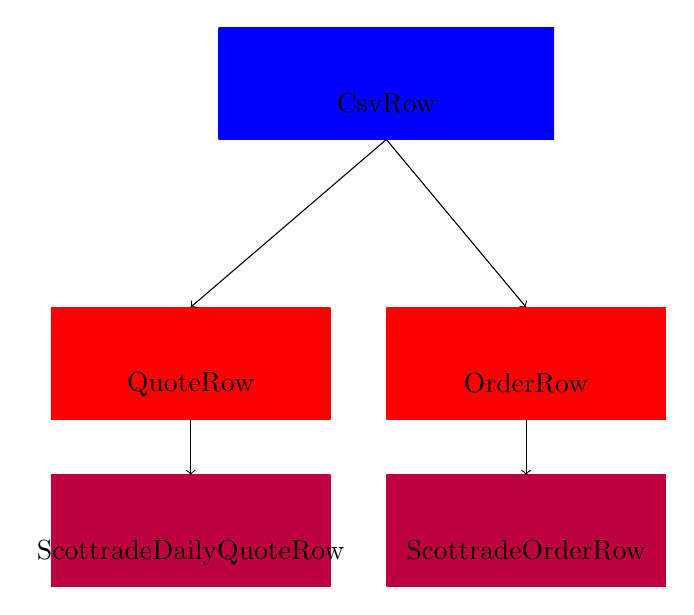
\begin{tikzpicture}[scale=0.71]
		\coordinate (B1_L) at (0,0);
		\coordinate (B1_R) at (5,2);
		\coordinate (B2_L) at (6,0);
		\coordinate (B2_R) at (11,2);
		\coordinate (B3_L) at (3,5);
		\coordinate (B3_R) at (9,7);
		\coordinate (B4_L) at (0,-3);
		\coordinate (B4_R) at (5,-1);
		\coordinate (B5_L) at (6,-3);
		\coordinate (B5_R) at (11,-1);

		\drawBox{B1_L}{B1_R}{QuoteRow}{red}{0}
		\drawBox{B2_L}{B2_R}{OrderRow}{red}{0}
		\drawBox{B3_L}{B3_R}{CsvRow}{blue}{0}
		\drawBox{B4_L}{B4_R}{ScottradeDailyQuoteRow}{purple}{0}
		\drawBox{B5_L}{B5_R}{ScottradeOrderRow}{purple}{0}
		\drawLinkArrowVertical {B3_L}{B3_R}{B1_L}{B1_R}
		\drawLinkArrowVertical {B3_L}{B3_R}{B2_L}{B2_R}
		\drawLinkArrowVertical {B1_L}{B1_R}{B4_L}{B4_R}
		\drawLinkArrowVertical {B2_L}{B2_R}{B5_L}{B5_R}

	\end{tikzpicture}
\end{frame}

\subsection{Projects-1 }
\begin{frame}
	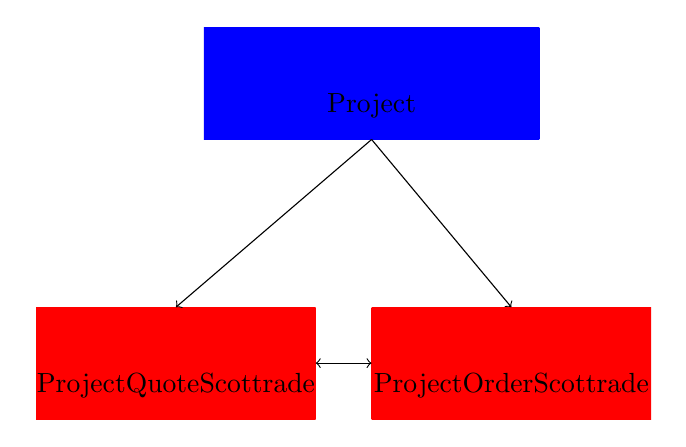
\begin{tikzpicture}[scale=0.71]
		\coordinate (B1_L) at (0,0);
		\coordinate (B1_R) at (5,2);
		\coordinate (B2_L) at (6,0);
		\coordinate (B2_R) at (11,2);
		\coordinate (B3_L) at (3,5);
		\coordinate (B3_R) at (9,7);

		\drawBox{B1_L}{B1_R}{ProjectQuoteScottrade}{red}{0}
		\drawBox{B2_L}{B2_R}{ProjectOrderScottrade}{red}{0}
		\drawBox{B3_L}{B3_R}{Project}{blue}{0}
		\drawLinkArrowVertical {B3_L}{B3_R}{B1_L}{B1_R}
		\drawLinkArrowVertical {B3_L}{B3_R}{B2_L}{B2_R}
		\drawLinkArrowHorizontal {B1_L}{B1_R}{B2_L}{B2_R}
	\end{tikzpicture}
\end{frame}

\subsection{Projects-2 }
\begin{frame}
	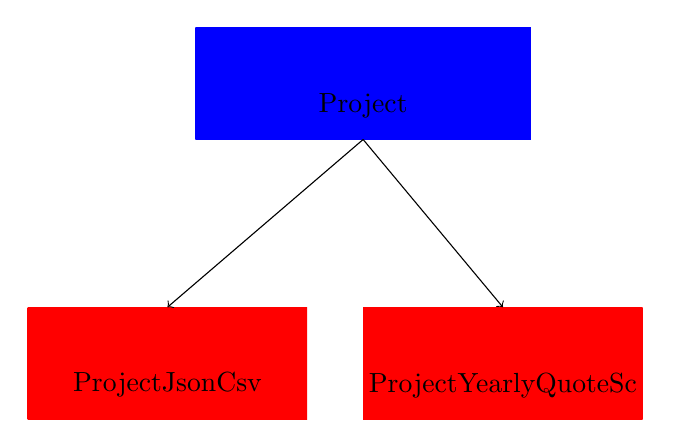
\begin{tikzpicture}[scale=0.71]
		\coordinate (B1_L) at (0,0);
		\coordinate (B1_R) at (5,2);
		\coordinate (B2_L) at (6,0);
		\coordinate (B2_R) at (11,2);
		\coordinate (B3_L) at (3,5);
		\coordinate (B3_R) at (9,7);

		\drawBox{B1_L}{B1_R}{ProjectJsonCsv}{red}{0}
		\drawBox{B2_L}{B2_R}{ProjectYearlyQuoteSc}{red}{0}
		\drawBox{B3_L}{B3_R}{Project}{blue}{0}
		\drawLinkArrowVertical {B3_L}{B3_R}{B1_L}{B1_R}
		\drawLinkArrowVertical {B3_L}{B3_R}{B2_L}{B2_R}
	\end{tikzpicture}
\end{frame}


\begin{frame}{ALl projects}
    \begin{itemize}
	\item Quotes (Scottrade) 
    		\begin{itemize}
			\item DailyQuotes
				This project ingests a daily quote file from scottrade and outputs the deserialized rows in specific format. We may append this deserialized form to an aggregate file.
			\item ConsumeAllDailyQuotes
				This project can process a whole dir of quotes files using \textbf{DailyQuotes} and append to aggegate file.
    		\end{itemize}
	\item Orders (Scottrade)
		This can ingest a order file and a daily quote file and produce the break up of losses and gains of past and present holdings. Holdings are grouped under symbols. We can split a single ticker as per their  purchase dates. 
	\item 

    \end{itemize}
\end{frame}

\begin{frame}{Daily Quote data structure}

    \begin{itemize}
	\item Think of data of all stocks as json file
	\item each data point belongs to a given stock and exchange
    		\begin{itemize}
			\item may contain time zone(utc implicit)
			\item current value at instant
			\item instant time stamp with tags like local,unix,utc,precision
			\item current volume at instant(normally this is day's volume from start of day.
			\item high ,low price
			\item open price and day's start timestamap(us start time only)
			\item day's end timestamp(us end time)
			\item previous working day's start timestamp ,end ts, volume, price,high ,low,open,close,percent change
		\end{itemize}
	\item each attribute has a default start at day. Volume starts with 0.Price starts with last closing price(in case available or current price if not available). Data structure should have this notion when storing. 
	\item a compendium of above data will make a total world. 
	
	\end{itemize}
	
\end{frame}

\begin{frame}{Daily Quote ops on data}

	\begin{itemize}
		\item find the graph on a given dimension
		\item sort data as per time stamp and project attributes 
		\item create csv files on any set of attributes and study it.
	\end{itemize}
\end{frame}


\begin{frame}{Daily Quotes project simplifying assumptions}
	\begin{itemize}
		\item days data instead of hourly data
	
	\end{itemize}
\end{frame}

\begin{frame}{Daily Quote rough implementation flow}
	\begin{itemize}
		\item we ingest a day's data.
		\item we append to an aggergate yearly file and corresponding entry meta file. Metafile is for deduplication.
		\item We can assume we have year loads of files containg day's data for years in past and current. The current year is still getting loaded.

		\item We can analyze these files for specific stock dumps. like dumping the flow data and analyzing it in python etc.
	\end{itemize}
\end{frame}


\begin{frame}{Order project}
	\begin{itemize}
		\item The order project checks current orders and prepares tranactions. Transaction is narrowly defined based on certain impl critrerias.
		\item Order project also depends on the quote project to get the latest quote of currently held stocks.
		\item We may need a csv project that can suitably render any json file produced by this project to a csv file based on  certain translation parameters may be provided as part of metadata.
		
	\end{itemize}
\end{frame}

\begin{frame}{CSV project}
	\begin{itemize}
		\item Read a arbirary json and convert it to csv
		\item arbitrary json will not be too arbitrary. There will be highest level arrays understood as rows.
		\item each row object will have only key value pairs. the value can be arbitrary object whose only one value can be displayed(this will be passed as metadata key).
		\item a DI map file for mpping fields fom json to csv should be provided and can be customized.
	\end{itemize}
\end{frame}

\begin{frame}{Yearly Analysis Project}
	\begin{itemize}
		\item Read a lots of  daily json file for all the stocks. Create yearly files of it.
		\item create a Time series  on some axis for each stock.
	\end{itemize}
\end{frame}



\end{document}

